\subsection{異部宗輪論}

\subsubsection{简介}
有關印度佛教史實之演化,佛滅以後,迄大乘盛行以前的大事,除結集而外,當以佛教部派的分化為最重要。
尤其在研究小乘佛教史之時,部派之分化一事,實為此時期的基本核心問題。
印度記載此一史實的史書,有《文殊師利問經》〈分部品〉,與《異部宗輪論》及其兩部同本異譯──《十八部論》與《部執異論》。
此即古來所稱小乘分派史料之「一經三論」。而此數書之中,當以《異部宗輪論》為最重要。
本論出於有部大家之作,故其主要內容,完全依照有部的說法來敘述,特別帶著北方有部正宗毗婆沙師的色彩。
論述佛滅後一百餘年(秦、陳譯本都作佛滅後一一六年)至四百年期間,印度佛教分派的歷史和各部派不同的教義(即部執)。
現有漢譯典籍,關於佛滅後佛教部派分裂次第以及各派異執的較完整的記述,僅有本論一種,所以它實為研究部派教義極重要的資料。

\subsubsection{译本}
\begin{itemize}
  \item 秦代的失譯本(A.D. 402~410?)《十八部論》一卷
  \item 陳.真諦(A.D. 545~569)譯《部執異論》一卷
  \item 唐.玄奘(A.D. 662)譯《異部宗輪論》一卷
\end{itemize}

\subsubsection{注解书}
\begin{itemize}
  \item 唐.窺基撰《異部宗輪論述記》一卷
  \item 憲榮撰《異部宗輪論述記發軔》共三冊
  \item 演培法師釋註《異部宗輪論語體釋》,諦觀全集論釋五。
\end{itemize}

\subsubsection{作者}
世友(Vasumitra),據玄奘所傳,係佛滅後四百年許迦膩色迦王時人,是當時說一切有部四大家之一。

\subsubsection{部派}
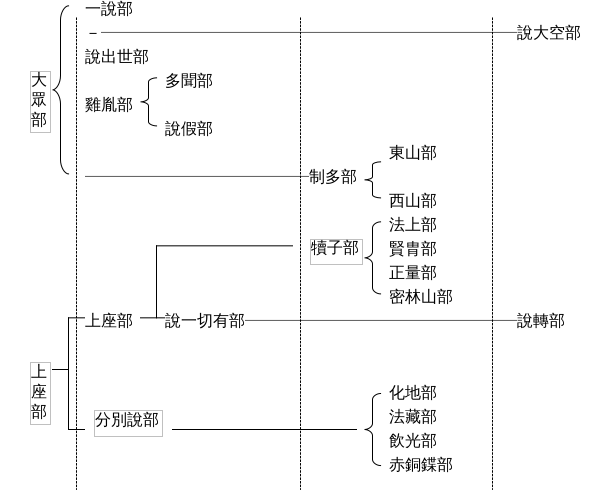
\includegraphics[scale=0.5]{Buddhism/images/部派佛教分化.png}

\subsubsection{地区分布}
\begin{itemize}
  \item 西北印度各地→說一切有部、經量部、大眾部、法藏部、化地部、飲光部。
 \item 西南印度和西印度地區→犢子部、正量部、法上部、賢胄部、密林山部(六城部)。
 \item 中印度至西北印度→大眾部、一說部、說出世部、雞胤部(牛家部)。
 \item 南印度之案達羅→制多山部、東山部、西山部、北山部、南方大眾部(大天派)。
 \item 北印度之雪山→根本上座部(雪山部)。
\end{itemize}

\subsubsection{四眾}
\begin{itemize}
  \item 龍象眾──優波離之徒    持律 \footnote{破戒僧所依.鬥諍之首}
	\item 邊鄙眾──大天之徒     破戒 \footnote{心行理外.聽說不能}
	\item 多聞眾──阿難之徒     誦經持佛語 \footnote{具戒依聞.凡夫}
	\item 大德眾──滿慈之徒     論師 \footnote{具智隨理.聖者}
\end{itemize}

\subsubsection{大天五事}
 餘所誘(Temptation by the other)
 \footnote{
「彼(大天)後既出在僧伽藍,不正思惟夢失不淨。然,彼先稱是阿羅漢,而令弟
子浣所污衣。弟子白言:『阿羅漢者諸漏已盡,師今何容猶有斯事?』大天告言:『天
魔所嬈,汝不應怪。然,所漏失略有二種:一者煩惱,二者不淨。煩惱漏失阿羅漢
無,猶未能免不淨漏失。所以者何?諸阿羅漢煩惱雖盡,豈無便利、涕唾等事。然,
諸天魔常於佛法而生憎嫉,見修善者便往壞之;縱阿羅漢亦為其嬈,故我漏失。是
彼所為,汝今不應有所疑怪。』是名第一惡見等起。」}

 無知(Ignorance)
\footnote{「又彼大天欲令弟子歡喜親附,矯設方便次第記別四沙門果。時,彼弟子稽首白言:
『阿羅漢等應有證智,如何我等都不自知?』彼遂告言:『諸阿羅漢亦有無知,汝
今不應於己不信,謂諸無知略有二種:一者染污,阿羅漢已無;二者不染污,阿羅
漢猶有。由此汝輩不能自知。』是名第二惡見等起。」}

 猶豫(Doubt)
\footnote{「時諸弟子復白彼言:『曾聞聖者已度疑惑,如何我等於諦實中猶懷疑惑?』彼
告言:『諸阿羅漢亦有疑惑!疑有二種:一者隨眠性疑,阿羅漢已斷;二者處非處
疑,阿羅漢未斷。獨覺於此而猶成就,況汝聲聞於諸諦實能無疑惑而自輕耶?』是
名第三惡見等起。」}

 他令入(Entrance through the other):
\footnote{「後彼弟子披讀諸經,說阿羅漢有聖慧眼,於自解脫能自證知。因白師言:『我等
若是阿羅漢者應自證知,如何但由師之令入都無現智能自證知?』彼即答言:『有
阿羅漢但由他入不能自知,如舍利子智慧第一、大目乾連神通第一。佛若未記彼不
自知,況由他入而能自了,故汝於此不應窮詰。』是名第四惡見等起。」}

 道因聲故起(The path arises through utterance)
\footnote{「然彼大天雖造眾惡,而不斷滅諸善根故,後於中夜自惟罪重,當於何處受諸劇苦,
憂惶所逼數唱苦哉。近住弟子聞之驚怪,晨朝參問,起居安不?大天答言:『吾甚
安樂。』弟子尋白:『若爾,昨夜何唱苦哉?』彼遂告言:『我呼聖道,汝不應怪,
謂諸聖道若不至誠稱苦,召命終不現起;故我昨夜數唱苦哉。』是名第五惡見等起。」}
